\documentclass{article}
\usepackage{lmodern}
\usepackage{graphicx} % Required for inserting images
\renewcommand{\thesubsection}{\arabic{subsection}}

\title{Peer review \#1 - GC11 - Model}
\author{Samuele Pischedda, Angelo Prete, Gabriele Raveggi, Andrea Sanvito }
\date{26/03/2024}

\begin{document}

\begin{titlepage}
\maketitle
\end{titlepage}

\section*{General Overview}
In this document we describe the UML of our Codex Naturalis java implementation. 
In particular, we will explain how we implemented the model of the MVC architectural pattern.
% TODO inserire png uml tutto
\begin{center}
    \hspace*{0.3cm}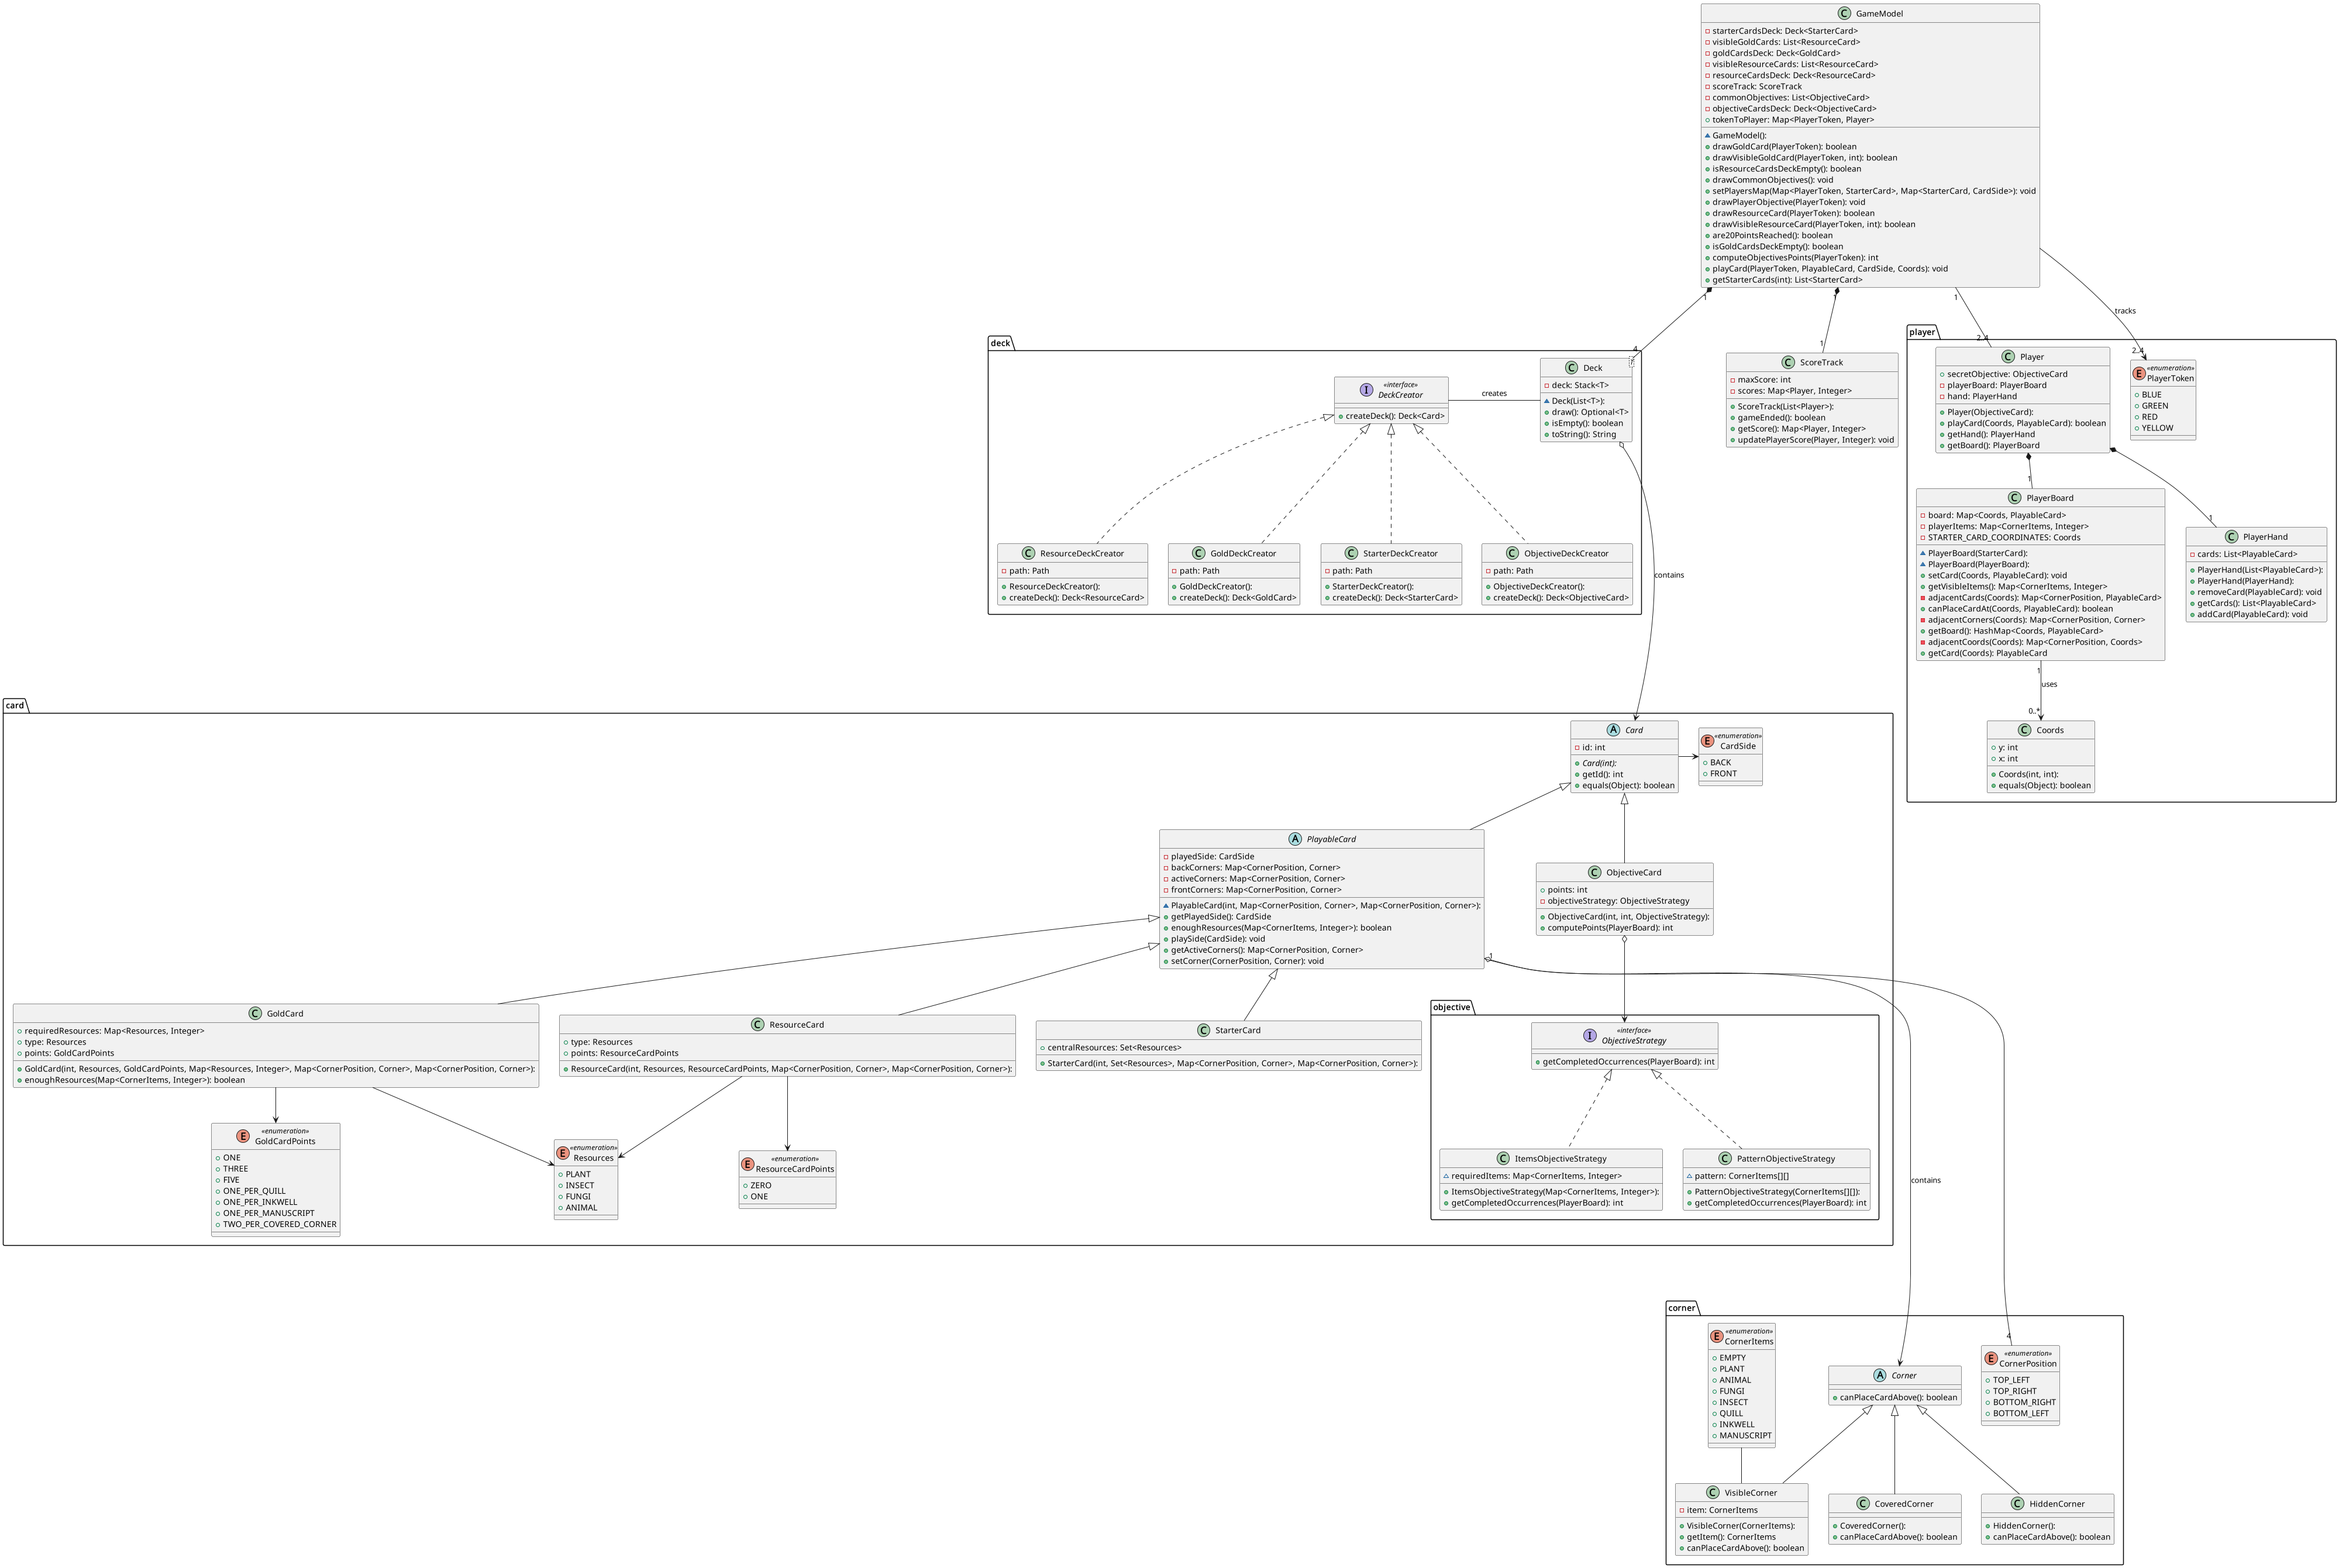
\includegraphics[scale=0.1]{model.png}
\end{center}


\newpage
\section*{Components description}
\setcounter{section}{1}
\subsection[1]{Class: \texttt{GameModel}}
The \texttt{GameModel} class is the core component of a game.
While it doesn't contain a finite state machine, which we will implement in the controller package and that will define the flow and behavior of a match, it holds the state of the match.
In fact, it contains numerous informations about the state of the different game entities:
\begin{itemize}
    \item a map defining the color picked by each player;
    \item all the decks found on the board (the gold, resource, objective and starter decks);
    \item the visible drawable cards and common objectives;
    \item the score board (\texttt{ScoreTrack}).
\end{itemize}
Moreover, it contains many methods that allow retrieving and modifying the state:
\begin{itemize}
    \item functions to use during the setup phase, allowing players to draw their starter card and pick their own token;
    \item functions to draw and play cards;
    \item a function to check if twenty points have been reached by a player;
    \item functions to check if the decks are empty.
\end{itemize}

\begin{center}
    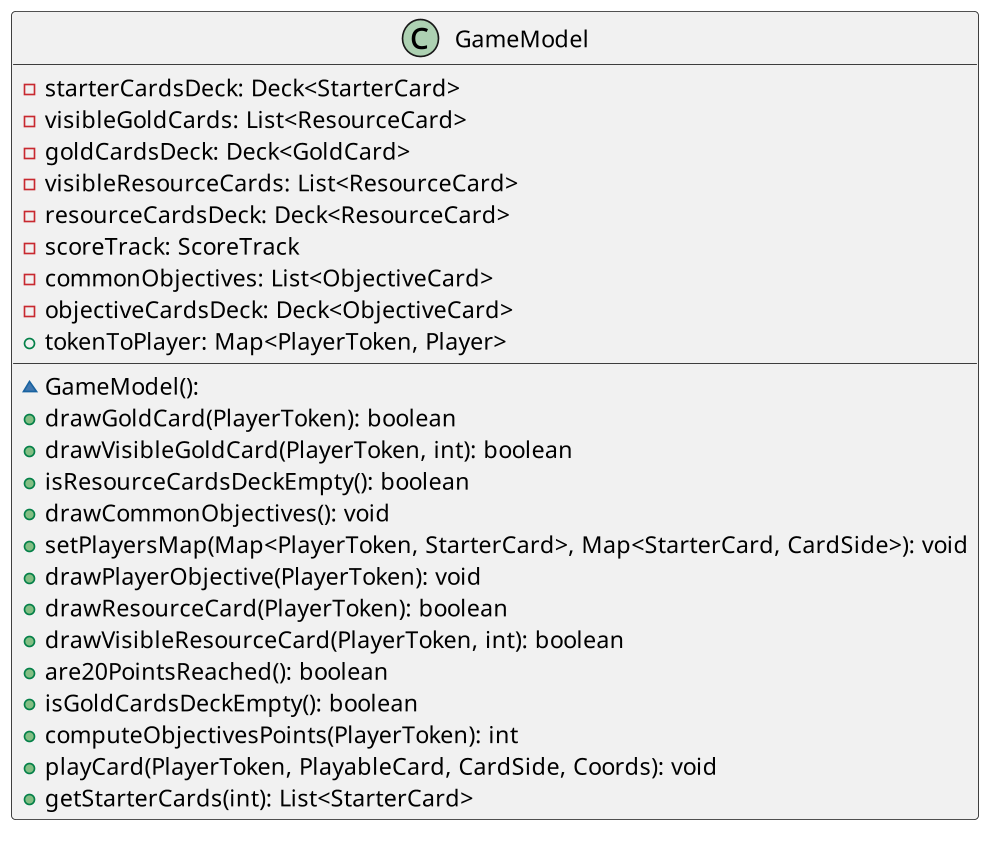
\includegraphics[scale=0.25]{GameModel.png}
\end{center}

\newpage
\subsection{Class: \texttt{ScoreTrack}}
This class tracks the individual scores of players.
In particular, it allows updating the score and checking if twenty points have been reached, through methods.

\begin{center}
    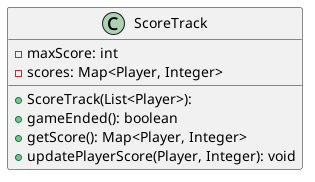
\includegraphics[scale=0.5]{ScoreTrack.png}
\end{center}
\newpage
\subsection{Package: \texttt{card}}
All the informations about cards and their properties are saved in this package.
Starting from the abstract class Card, two different subclasses are derived:
\begin{itemize}
    \item \texttt{ObjectiveCard}, that comes with its own \texttt{objective} package, implements the strategy pattern used to easily define different ways of computing points for objective cards;
    \item \texttt{PlayableCard} (abstract), that contains maps that track card corners' properties (explained later in the card package). 
    The \texttt{PlayableCard} class is divided into the following subclasses (each with their own properties):
    \begin{itemize}
        \item \texttt{ResourceCard};
        \item \texttt{GoldCard};
        \item \texttt{StarterCard}.
    \end{itemize}
\end{itemize}
This package also contains the enumerations needed to represent each propery:
\begin{itemize}
    \item \texttt{CardSide};
    \item \texttt{Resources};
    \item \texttt{ResourceCardPonts};
    \item \texttt{GoldCardPoints}.
\end{itemize}

\begin{center}
    \hspace*{-3cm}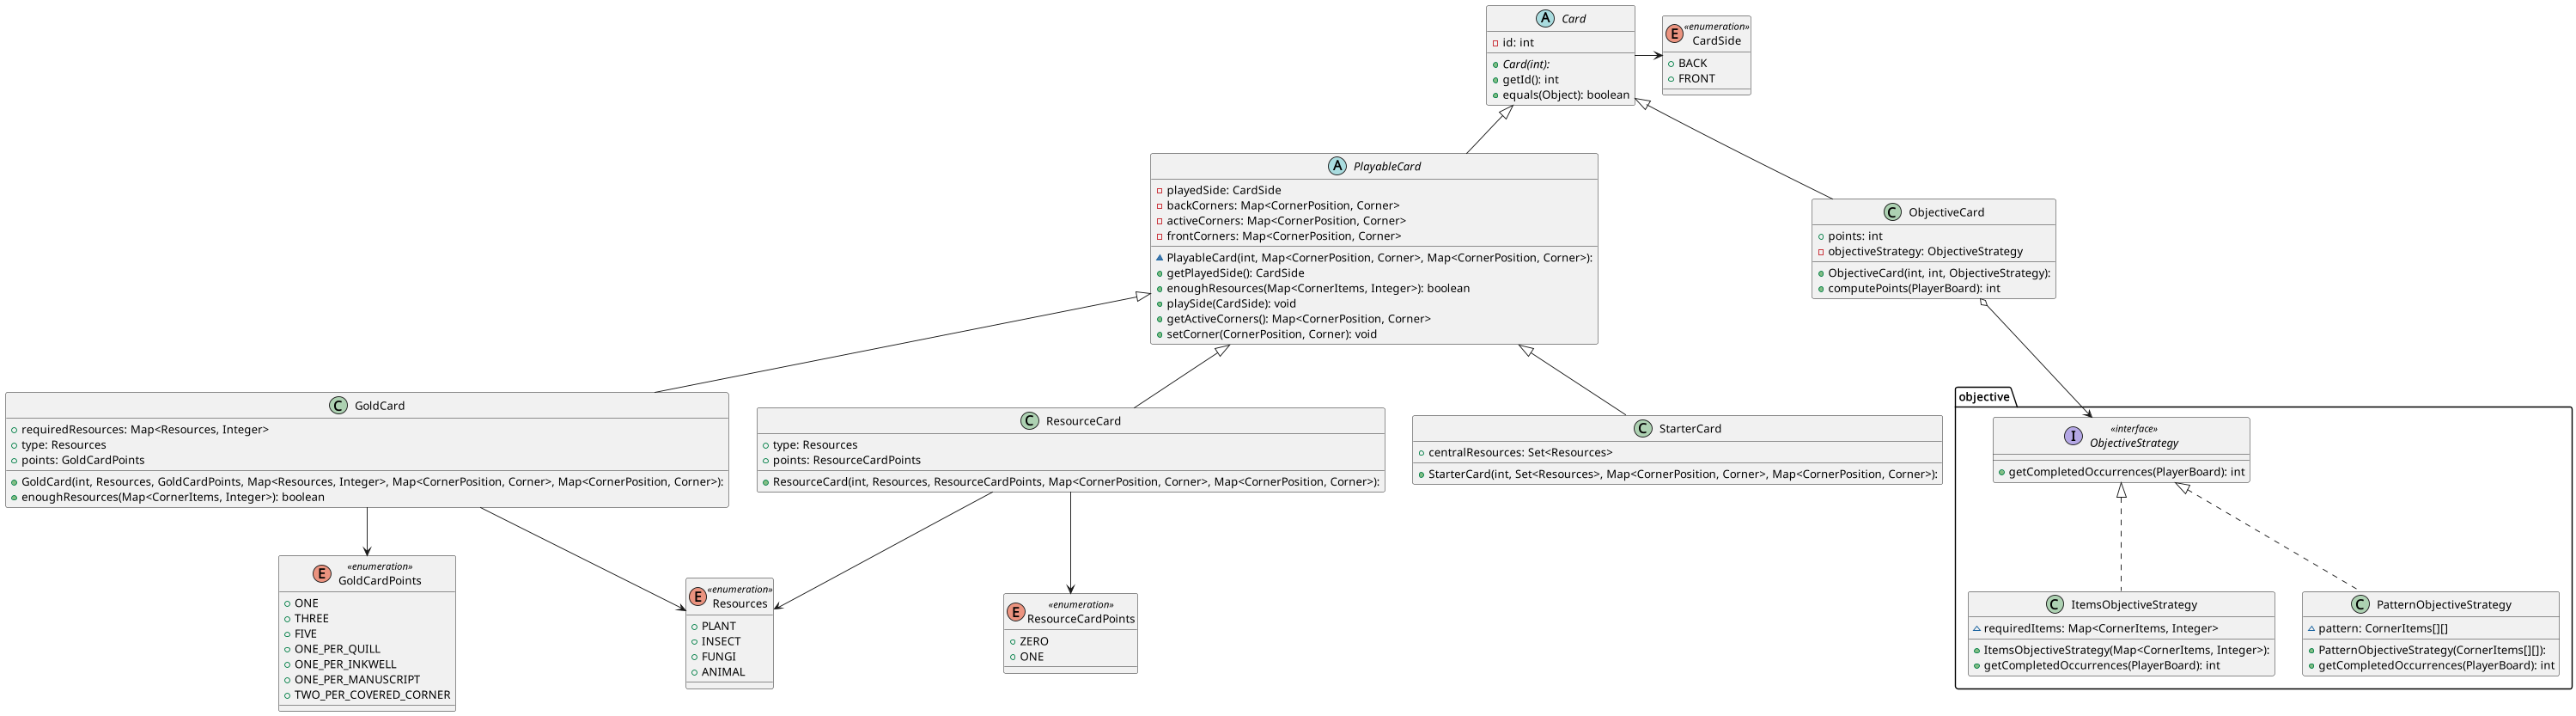
\includegraphics[scale=0.18]{card.png}
\end{center}
\newpage
\noindent

\subsection{Package: \texttt{deck}}
The package contains a main generic \texttt{Deck} class, which implements a deck as a stack of a generic card type.
It is used in the \texttt{GameModel} class, to represent the different decks used during the game. 
Furthermore, using the factory method pattern we load the decks into the \texttt{GameModel} from json files.

\noindent For every card type, we initialize its deck through different deck creators, each implementing a common \texttt{DeckCreator} interface:
\begin{itemize}
    \item \texttt{GoldDeckCreator}
    \item \texttt{ObjectiveDeckCreator}
    \item \texttt{ResourceDeckCreator}
    \item \texttt{StarterDeckCreator}
\end{itemize}

\begin{center}
    \hspace*{-1cm}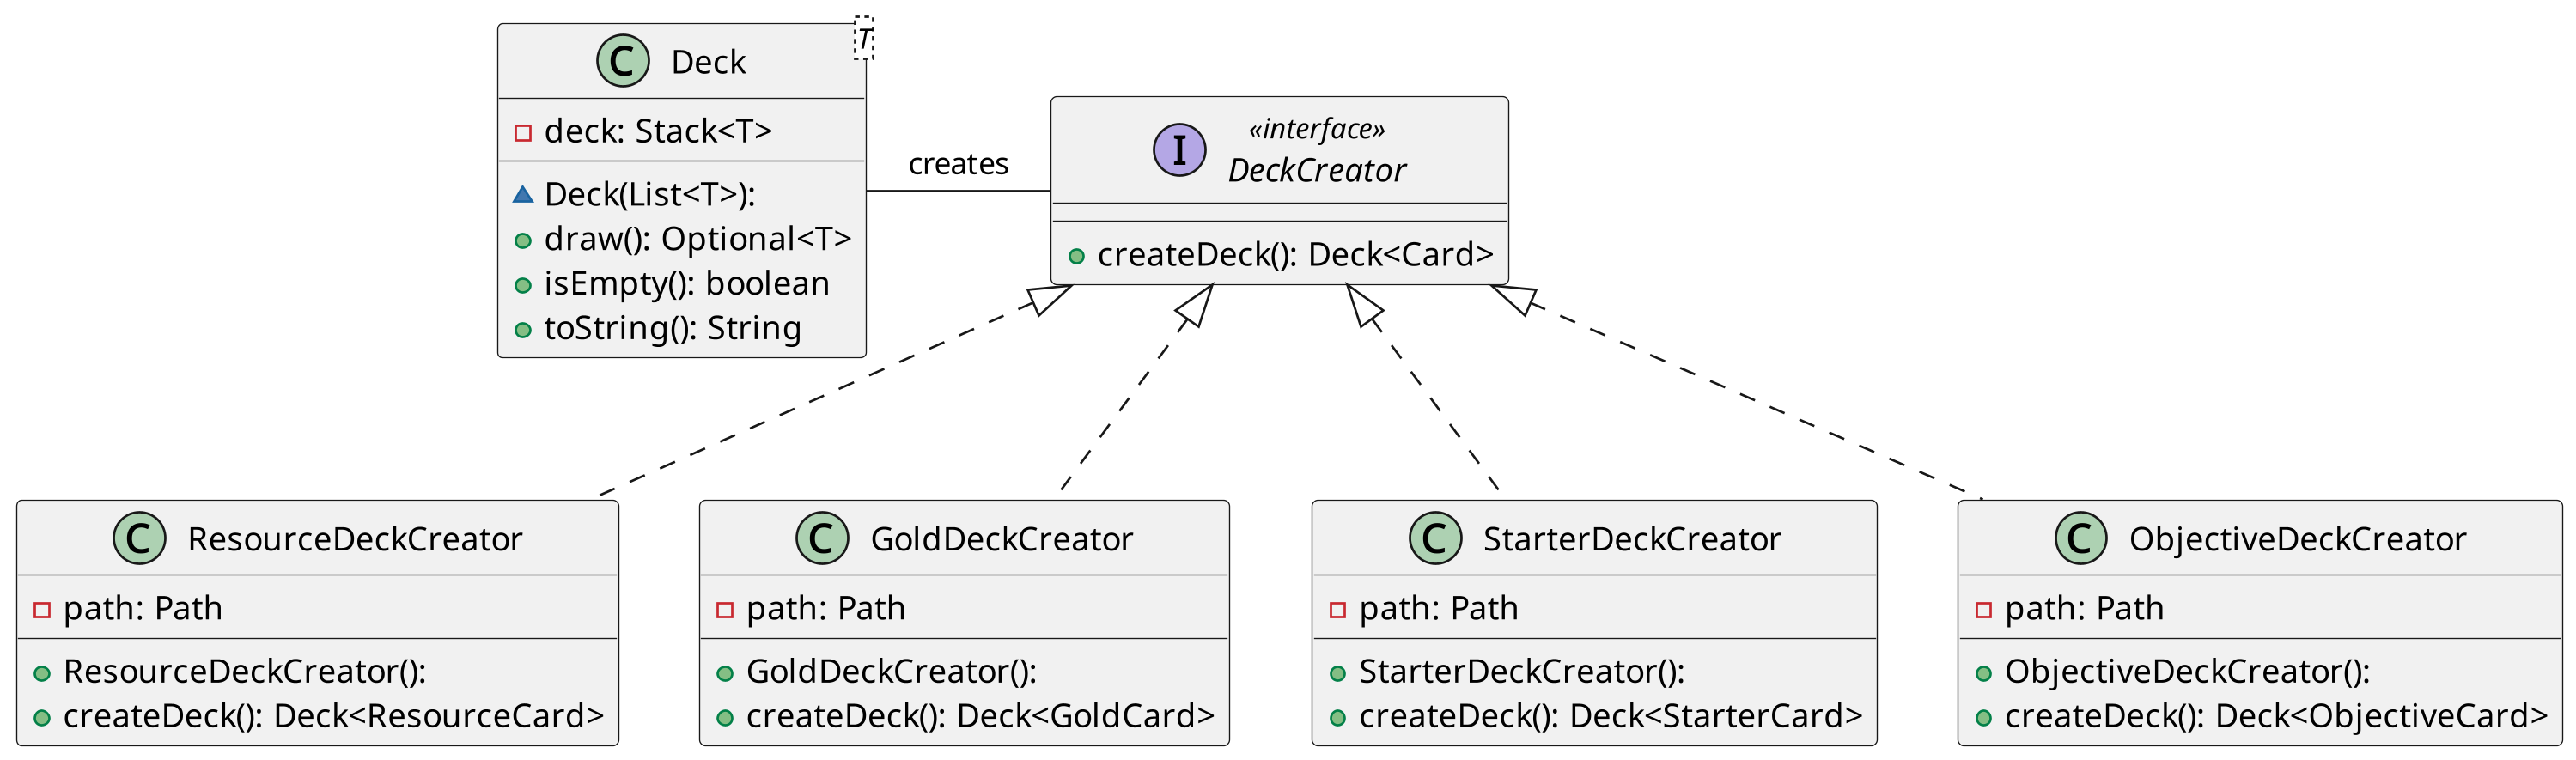
\includegraphics[scale=0.15]{deck.png}
\end{center}

\newpage
\subsection{Package: \texttt{corner}}
The package includes an abstract \texttt{Corner} class which represents a generic corner of a card.
The main class is extended by the following classes:
\begin{itemize}
    \item \texttt{CoveredCorner}: a corner of a card that has been covered by another card, thus it is not visible;
    \item \texttt{HiddenCorner}; a missing corner (hidden), where you can't place any card;
    \item \texttt{VisibleCorner}: a corner of a card that is either empty or contains an item.
\end{itemize}
To keep track of the position of a corner in a card, we use the \texttt{CornerPosition} enum.
\noindent
The \texttt{CornerItems} enum is used to represent an item in a visible corner.
\begin{center}
    \hspace*{-2cm}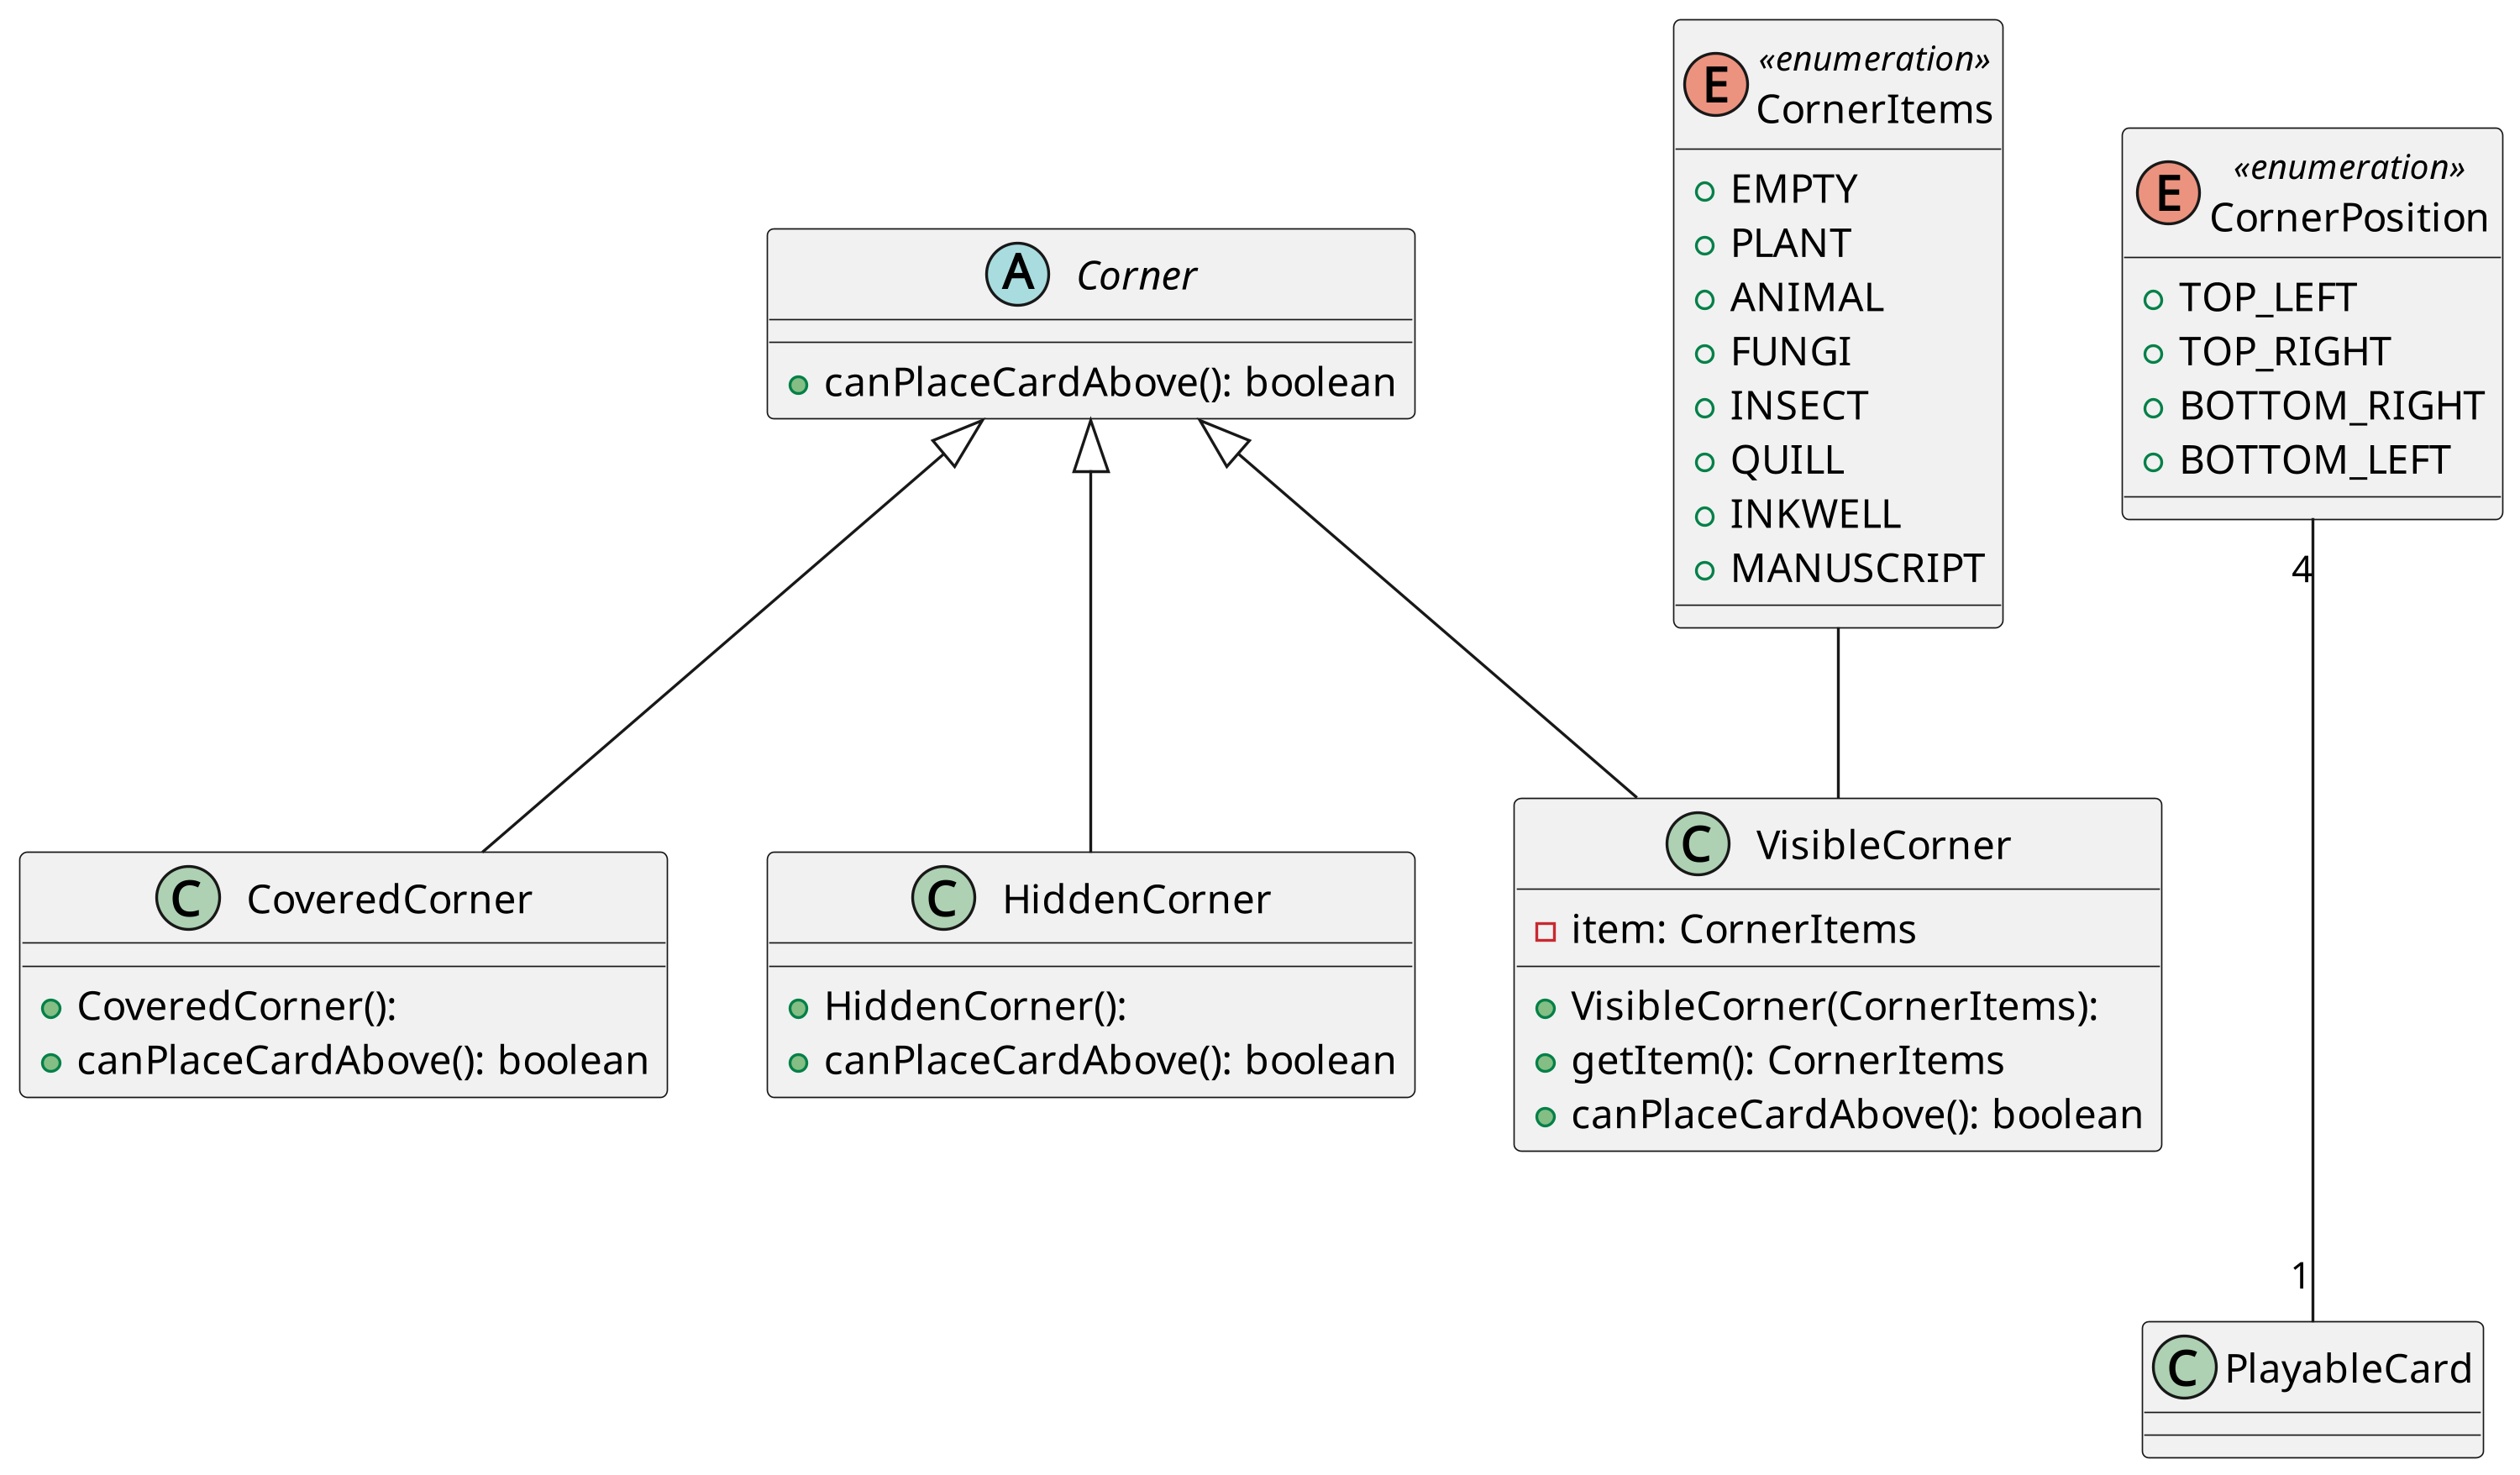
\includegraphics[scale=0.15]{corner.png}
\end{center}

\newpage
\subsection{Package: \texttt{player}}
The package contains a main \texttt{Player} class which represents a single player in the game.
The player class contains different attributes to identify their game entities:
\begin{itemize}
    \item a \texttt{PlayerBoard} object that models the board of the player;
    \item a \texttt{PlayerHand} object that represents the three cards in a player hand;
    \item the \texttt{ObjectiveCard} secret objetive.
\end{itemize}

\noindent
More specifically, the other classes are:
\begin{itemize}
    \item \texttt{PlayerBoard}: contains two maps, one to model the player's board, and one to keep track of the amount of visible items by item type;
    \item \texttt{PlayerHand}: implemented as a list of \texttt{PlayableCard};
    \item \texttt{Coords}: represents 2D coordinates that can be used to identify cards' position in the player board.
\end{itemize}
\noindent
The package also contains the PlayerToken enumeration, used to represent a single player in the model side of the project thanks to a mapping in the GameModel.

\begin{center}
    \hspace*{-2cm}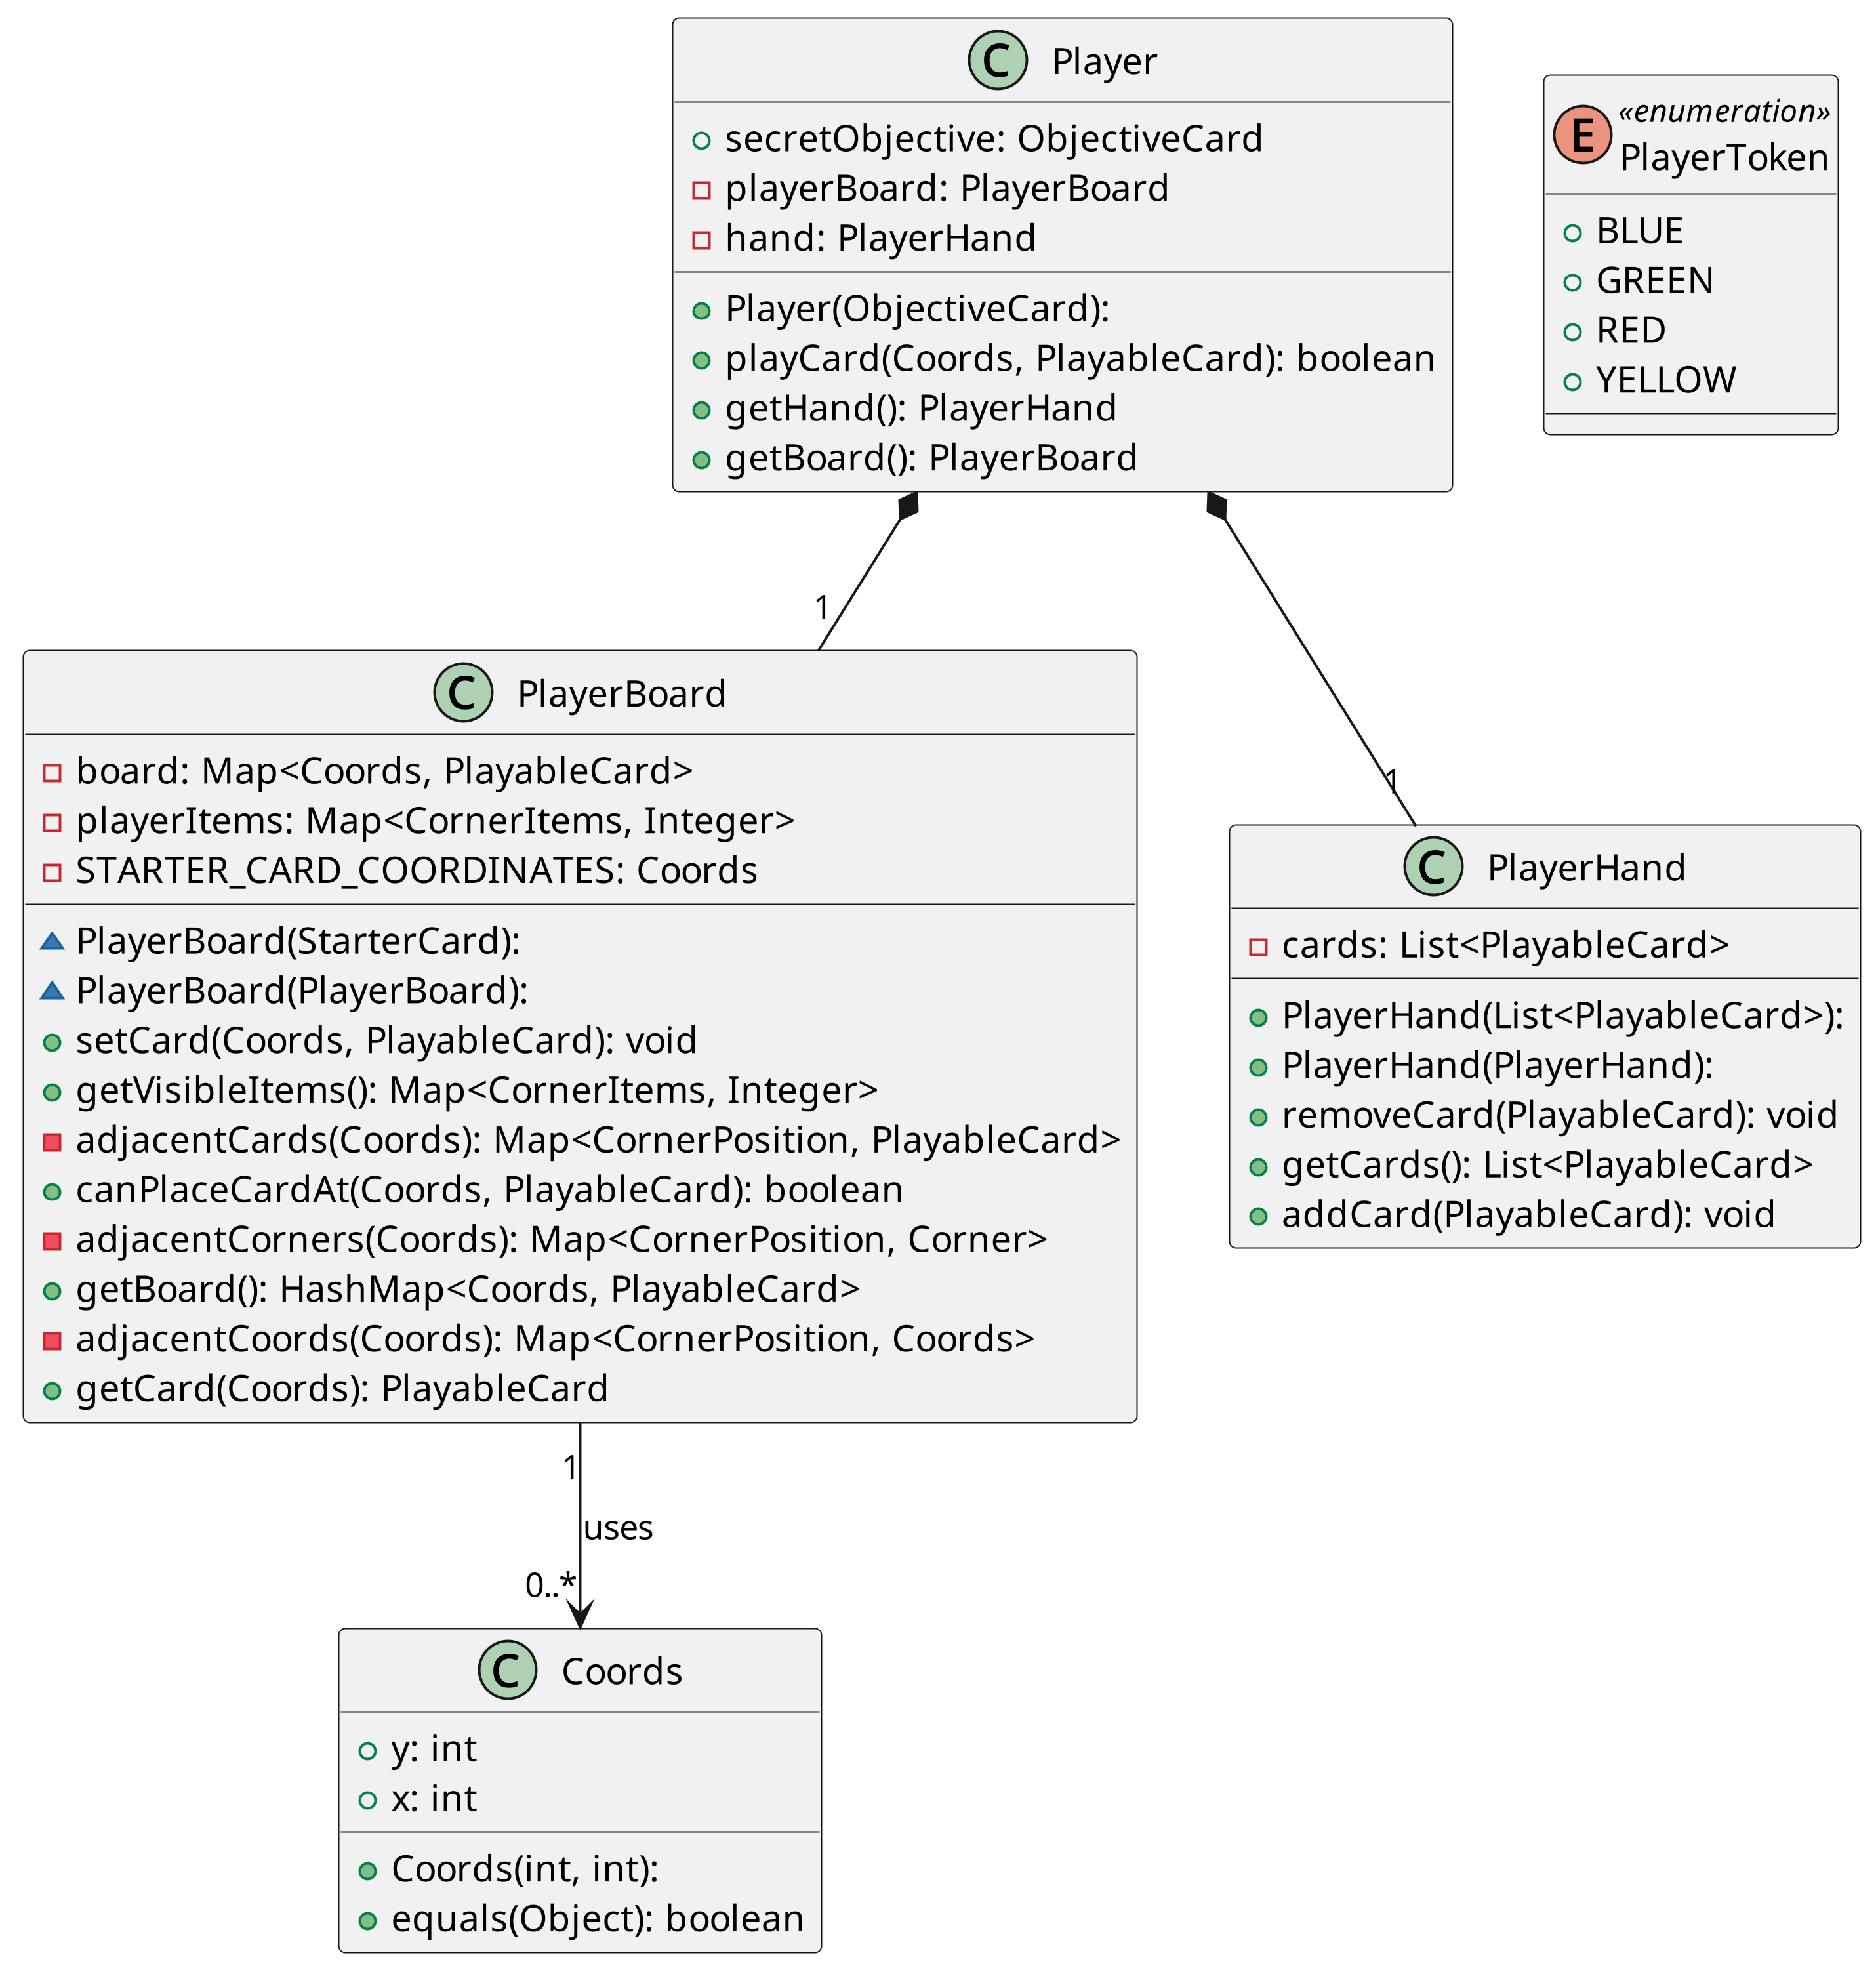
\includegraphics[scale=0.1]{player.png}
\end{center}
\end{document}